\chapter{Microservizio anagrafica}

\section{Scopo del sistema}

Il sistema di anagrafica si occupa di gestire le informazioni anagrafiche dei sensori, delle aree e dei lampioni. Gestisce questi raggruppamenti e si occupa di renderli persistenti su database.

\section{Requisiti coperti dal sistema}

\section{Descrizione del sistema}

Il sistema principalmente fornisce le informazioni stoccate su base dati tramite un'interfaccia rest.
Questo è poi in grado di fornire i dati in forma aggregata, come ad esempio il numero di lampioni per area, o il numero di sensori per lampioni.

Per queste informazioni ha inoltre il compito e la responsabilità di tenere aggiornati i dati nel database.

\section{Architettura del sistema}

L'architettura base del sistema è in MVVM. Non è presente la necessità di multi input e multi output, quindi non è necessario utilizzare un'architettura esagonale come nel caso del sistema di autenticazione.

I componenti del programma sono quindi divisi in tre parti: Model, View e ViewModel.

\begin{figure}[h]
    \centering
    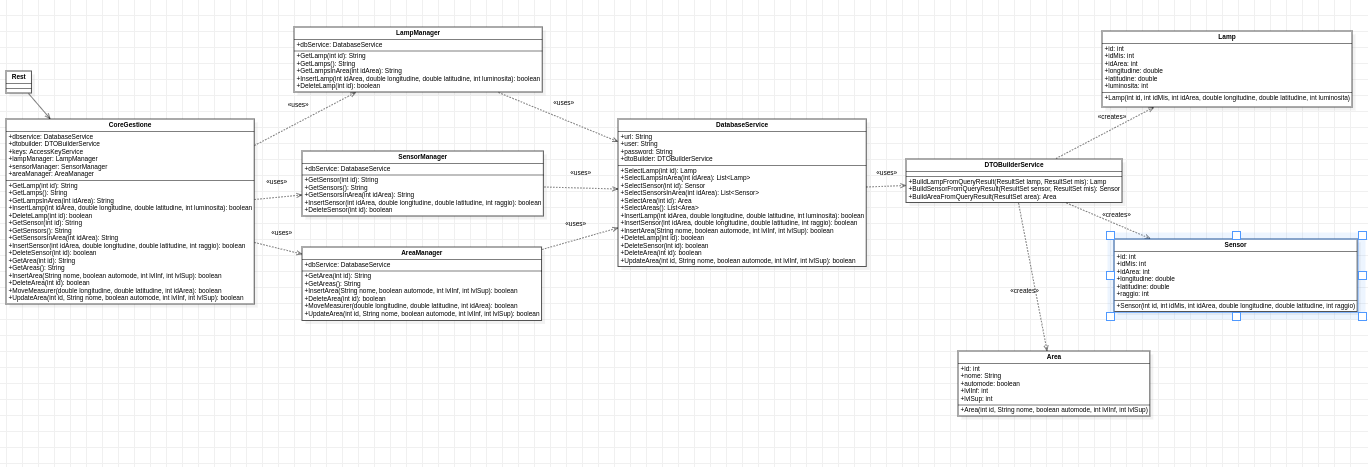
\includegraphics[width=\textwidth]{img/anagrafe_generale.png}
    \caption{Vista generale del sistema di anagrafe}
    \label{fig:general_anagrafe}
\end{figure}


\begin{figure}[h]
    \centering
    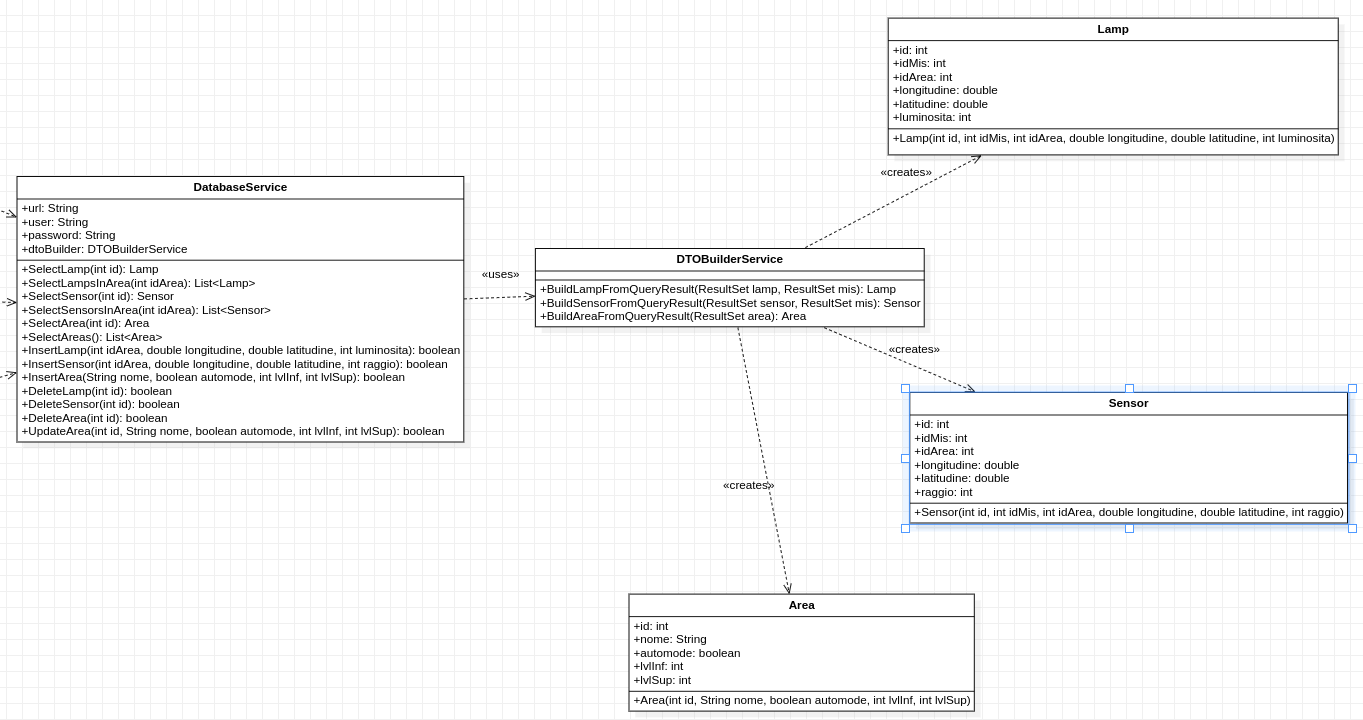
\includegraphics[width=\textwidth]{img/model_anagrafe.png}
    \caption{Diagramma delle classi del modello all'interno del sistema di anagrafe}
    \label{fig:model_anagrafe}
\end{figure}




